\documentclass[12pt,nohyper]{tufte-handout}\usepackage[]{graphicx}\usepackage[]{color}
%% maxwidth is the original width if it is less than linewidth
%% otherwise use linewidth (to make sure the graphics do not exceed the margin)
\makeatletter
\def\maxwidth{ %
  \ifdim\Gin@nat@width>\linewidth
    \linewidth
  \else
    \Gin@nat@width
  \fi
}
\makeatother

\definecolor{fgcolor}{rgb}{0.345, 0.345, 0.345}
\newcommand{\hlnum}[1]{\textcolor[rgb]{0.686,0.059,0.569}{#1}}%
\newcommand{\hlstr}[1]{\textcolor[rgb]{0.192,0.494,0.8}{#1}}%
\newcommand{\hlcom}[1]{\textcolor[rgb]{0.678,0.584,0.686}{\textit{#1}}}%
\newcommand{\hlopt}[1]{\textcolor[rgb]{0,0,0}{#1}}%
\newcommand{\hlstd}[1]{\textcolor[rgb]{0.345,0.345,0.345}{#1}}%
\newcommand{\hlkwa}[1]{\textcolor[rgb]{0.161,0.373,0.58}{\textbf{#1}}}%
\newcommand{\hlkwb}[1]{\textcolor[rgb]{0.69,0.353,0.396}{#1}}%
\newcommand{\hlkwc}[1]{\textcolor[rgb]{0.333,0.667,0.333}{#1}}%
\newcommand{\hlkwd}[1]{\textcolor[rgb]{0.737,0.353,0.396}{\textbf{#1}}}%

\usepackage{framed}
\makeatletter
\newenvironment{kframe}{%
 \def\at@end@of@kframe{}%
 \ifinner\ifhmode%
  \def\at@end@of@kframe{\end{minipage}}%
  \begin{minipage}{\columnwidth}%
 \fi\fi%
 \def\FrameCommand##1{\hskip\@totalleftmargin \hskip-\fboxsep
 \colorbox{shadecolor}{##1}\hskip-\fboxsep
     % There is no \\@totalrightmargin, so:
     \hskip-\linewidth \hskip-\@totalleftmargin \hskip\columnwidth}%
 \MakeFramed {\advance\hsize-\width
   \@totalleftmargin\z@ \linewidth\hsize
   \@setminipage}}%
 {\par\unskip\endMakeFramed%
 \at@end@of@kframe}
\makeatother

\definecolor{shadecolor}{rgb}{.97, .97, .97}
\definecolor{messagecolor}{rgb}{0, 0, 0}
\definecolor{warningcolor}{rgb}{1, 0, 1}
\definecolor{errorcolor}{rgb}{1, 0, 0}
\newenvironment{knitrout}{}{} % an empty environment to be redefined in TeX

\usepackage{alltt}
\usepackage[T1]{fontenc}
\usepackage[latin9]{inputenc}
\usepackage{wrapfig}
\usepackage{longtable}
\usepackage{hyperref}
\usepackage{graphicx}
\usepackage[space]{grffile}

\makeatletter
\makeatother
\IfFileExists{upquote.sty}{\usepackage{upquote}}{}
\begin{document}



\centerline{\Large\bf Statistics 101 Analysis for Section AB}
\centerline{\bf Homework Comparison across Topics 3 -- 6}
\centerline{\bf }


\section{Overview}

The 2 homework outcome files are Topic03.AB.csv, Topic06.AB.csv.


There are 50 students in Section AB 
submitting their answers. 50
of them did all the homeworks. Since different homeworks have different full 
scores, the percentages correct are used to compare among homeworks.
The average correct percents for the 2 homeworks are 
24, 25, respectively.
Figure \ref{mar:hist} compares the histograms of those homeworks.
Table \ref{tab:summary} and Figure \ref{fig:boxplot} display the basic summaries of the scores.


\begin{marginfigure}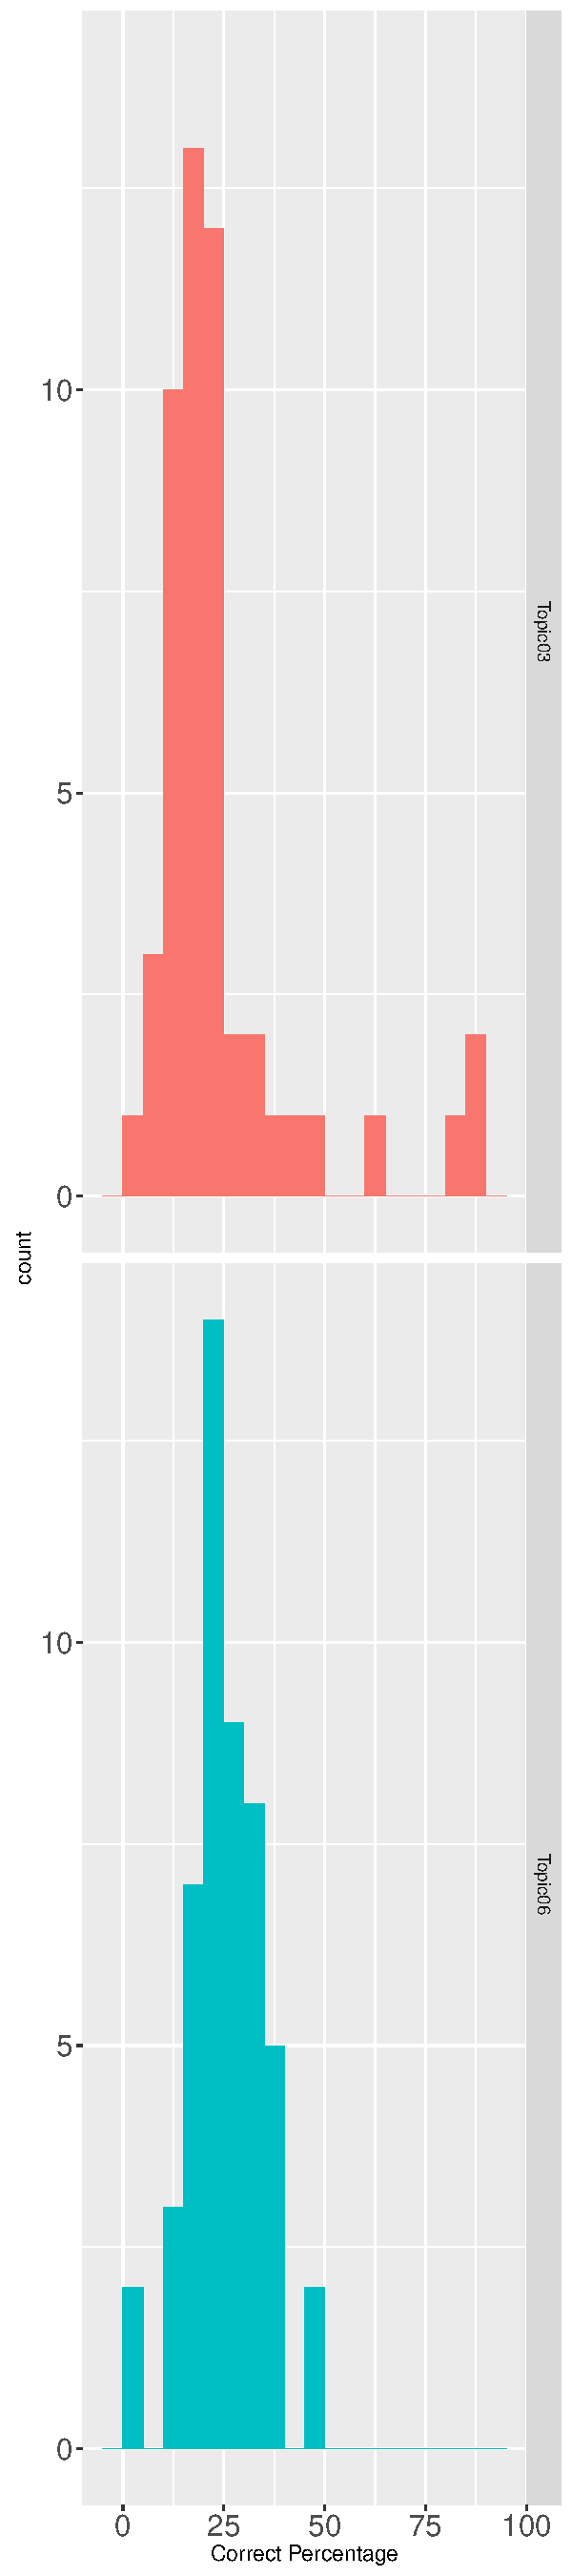
\includegraphics[width=0.95\linewidth]{Stat101_SectionAB_histbystu}
\caption{\label{mar:hist}Histograms of the percentages correct by students homeworks.}\end{marginfigure}% latex table generated in R 3.2.2 by xtable 1.8-0 package
% Sat Jan 16 13:39:57 2016
\begin{longtable}{rrrrrrrr}
  \hline
 & Mean & Std.dev &   &   & Min & Median & Max \\ 
  \hline
Topic03 & 23.80 & 18.74 &  &  & 0.00 & 17.14 & 88.57 \\ 
  Topic06 & 24.96 & 9.51 &  &  & 0.00 & 24.00 & 48.00 \\ 
   \hline
\hline
\caption{Summary statistics for correct percentage. Topic06 has the highest mean correct percentage, while Topic03 has the lowest. Topic03 has the largest standard deviation, and Topic06 has the smallest.} 
\label{tab:summary}
\end{longtable}


\clearpage

\begin{center}
\begin{wrapfigure}{o}{0.9\columnwidth}
\begin{centering}
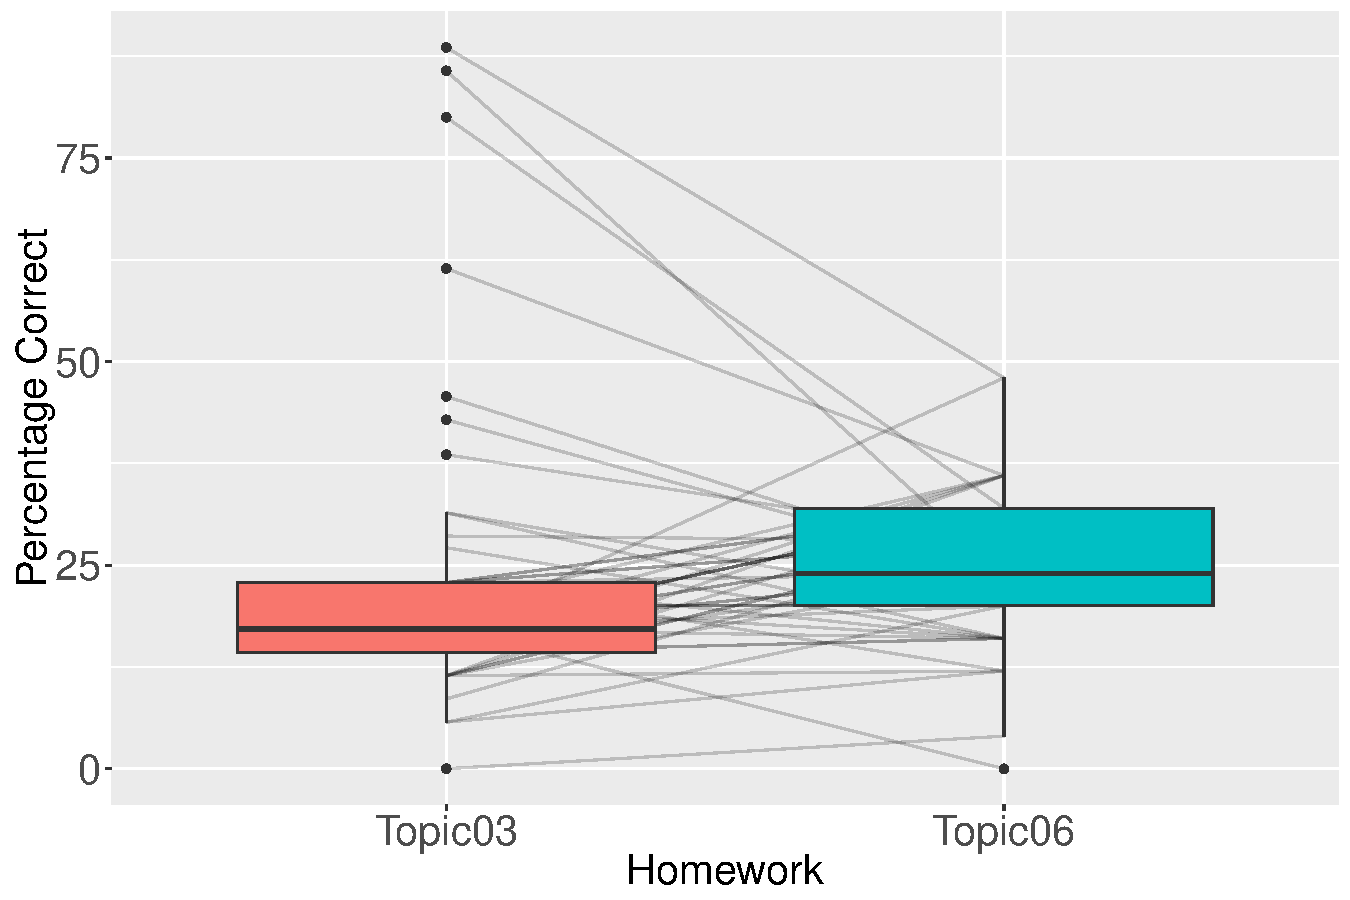
\includegraphics[width=0.9\linewidth]{Stat101_SectionAB_boxplotbystu}
\par\end{centering}
\caption{\label{fig:boxplot}Side-by-side boxplots of the percentages correct by students homeworks. Topic06 has the highest median, while Topic03 has the lowest median.}
\end{wrapfigure}\par\end{center}

\clearpage
\newpage{}
\section{Students}

Figure \ref{fig:heatmap} and Table \ref{tab:data} give the percentage
scores of each homework of all homeworks for every student in this section.
Table \ref{tab:data} also provides the mean percentages by student.
The students are sorted by their average percentage score of 2
homeworks. Table \ref{tab:lag} lists the students who were in the lower
20\% of the class.


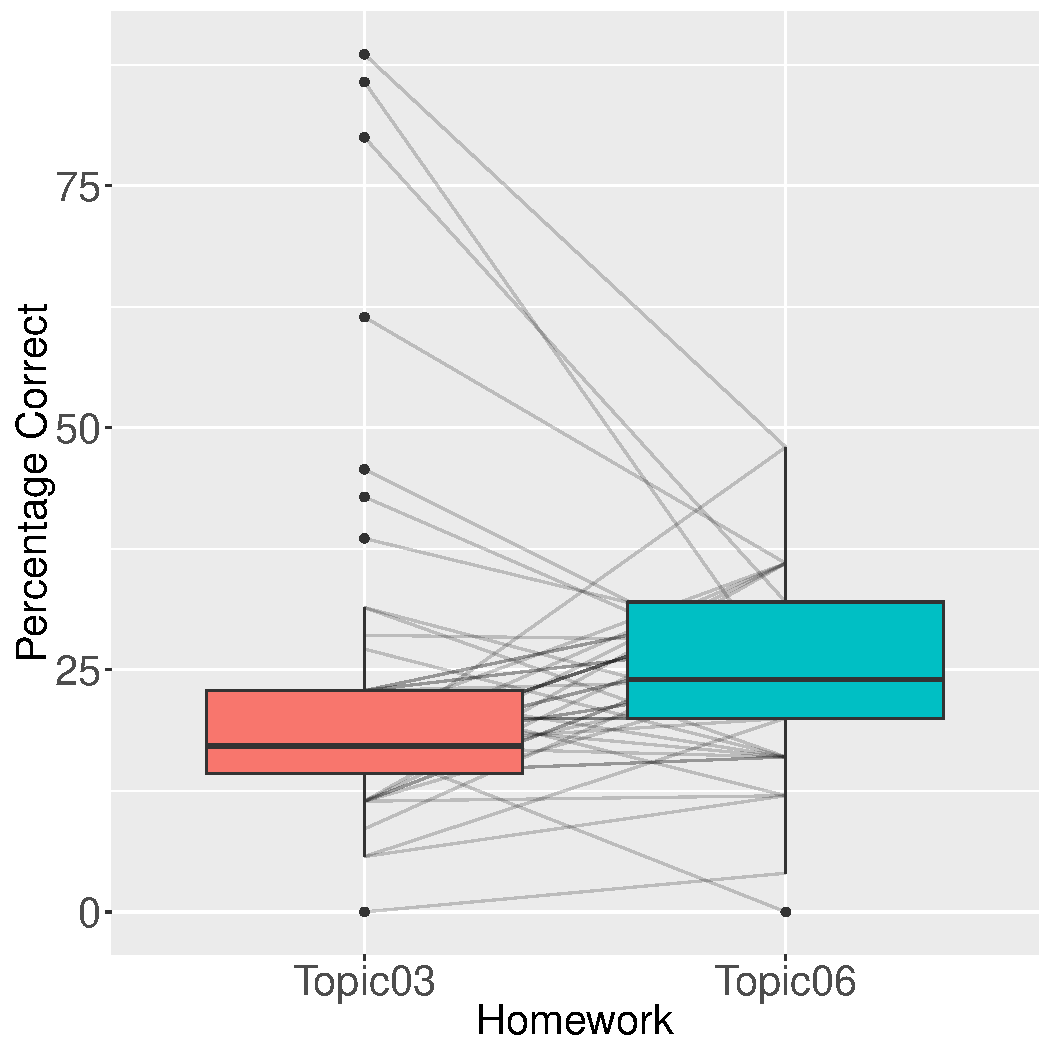
\includegraphics[width=\maxwidth]{figure/unnamed-chunk-4-1} 
\begin{center}
\begin{wrapfigure}{o}{0.95\columnwidth}
\begin{centering}
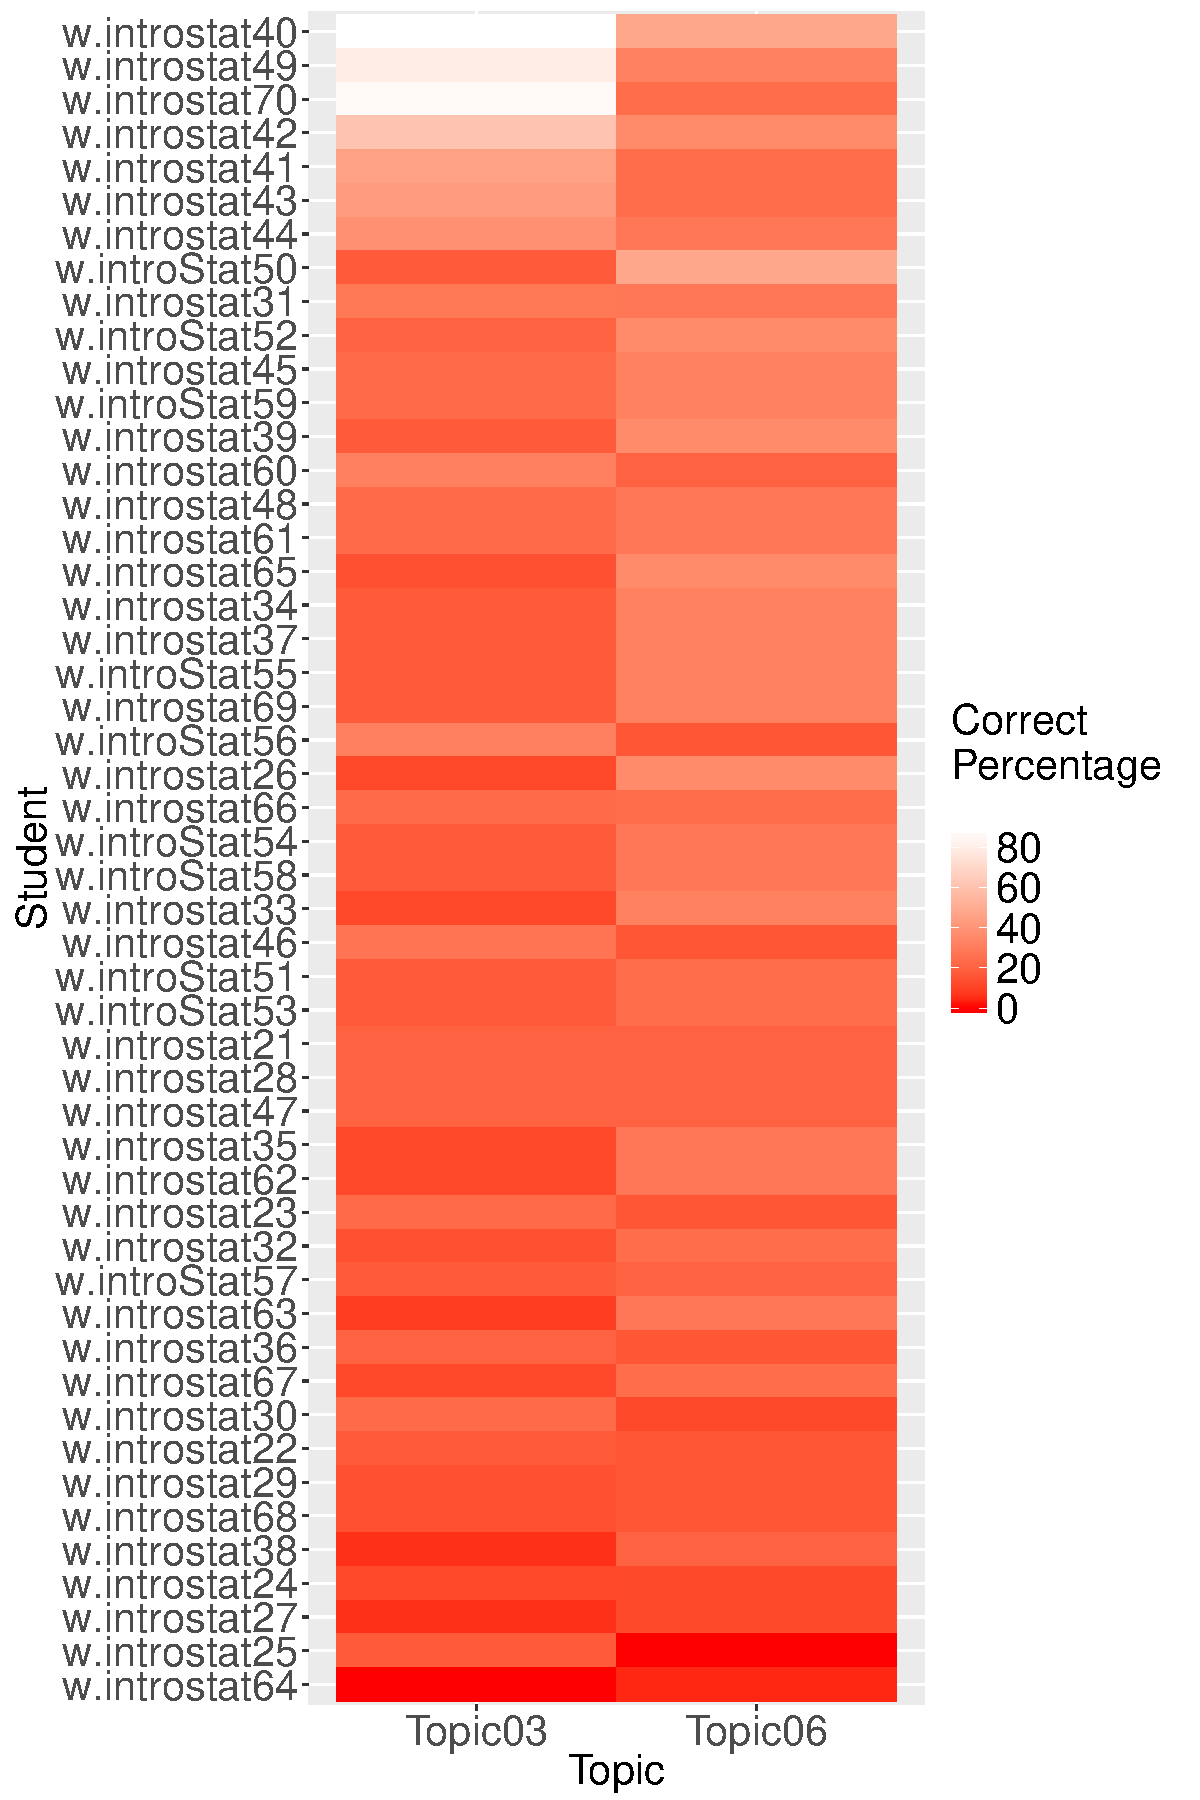
\includegraphics[width=0.99\linewidth]{Stat101_SectionAB_tile_student_topic}
\par\end{centering}
\caption{\label{fig:heatmap}Heatmap of the percentage scores of all homeworks for students in the section. The grey areas are the missing values.}
\end{wrapfigure}\par\end{center}

\clearpage

% latex table generated in R 3.2.2 by xtable 1.8-0 package
% Sat Jan 16 13:39:58 2016
\begin{longtable}{rrrr}
  \hline
 & Topic03 & Topic06 & AvgCrtPct \\ 
  \hline
w.introstat40 & 88.57 & 48.00 & 68.29 \\ 
  w.introstat49 & 80.00 & 32.00 & 56.00 \\ 
  w.introstat70 & 85.71 & 24.00 & 54.86 \\ 
  w.introstat42 & 61.43 & 36.00 & 48.71 \\ 
  w.introstat41 & 45.71 & 24.00 & 34.86 \\ 
  w.introstat43 & 42.86 & 24.00 & 33.43 \\ 
  w.introstat44 & 38.57 & 28.00 & 33.29 \\ 
  w.introStat50 & 17.14 & 48.00 & 32.57 \\ 
  w.introstat31 & 28.57 & 28.00 & 28.29 \\ 
  w.introStat52 & 20.00 & 36.00 & 28.00 \\ 
  w.introstat45 & 22.86 & 32.00 & 27.43 \\ 
  w.introStat59 & 22.86 & 32.00 & 27.43 \\ 
  w.introstat39 & 17.14 & 36.00 & 26.57 \\ 
  w.introstat60 & 31.43 & 20.00 & 25.71 \\ 
  w.introstat48 & 22.86 & 28.00 & 25.43 \\ 
  w.introstat61 & 22.86 & 28.00 & 25.43 \\ 
  w.introstat65 & 14.29 & 36.00 & 25.14 \\ 
  w.introstat34 & 17.14 & 32.00 & 24.57 \\ 
  w.introstat37 & 17.14 & 32.00 & 24.57 \\ 
  w.introStat55 & 17.14 & 32.00 & 24.57 \\ 
  w.introstat69 & 17.14 & 32.00 & 24.57 \\ 
  w.introStat56 & 31.43 & 16.00 & 23.71 \\ 
  w.introstat26 & 11.43 & 36.00 & 23.71 \\ 
  w.introstat66 & 22.86 & 24.00 & 23.43 \\ 
  w.introStat54 & 17.14 & 28.00 & 22.57 \\ 
  w.introStat58 & 17.14 & 28.00 & 22.57 \\ 
  w.introstat33 & 11.43 & 32.00 & 21.71 \\ 
  w.introstat46 & 27.14 & 16.00 & 21.57 \\ 
  w.introStat51 & 17.14 & 24.00 & 20.57 \\ 
  w.introStat53 & 17.14 & 24.00 & 20.57 \\ 
  w.introstat21 & 20.00 & 20.00 & 20.00 \\ 
  w.introstat28 & 20.00 & 20.00 & 20.00 \\ 
  w.introstat47 & 20.00 & 20.00 & 20.00 \\ 
  w.introstat35 & 11.43 & 28.00 & 19.71 \\ 
  w.introstat62 & 11.43 & 28.00 & 19.71 \\ 
  w.introstat23 & 22.86 & 16.00 & 19.43 \\ 
  w.introstat32 & 14.29 & 24.00 & 19.14 \\ 
  w.introStat57 & 17.14 & 20.00 & 18.57 \\ 
  w.introstat63 & 8.57 & 28.00 & 18.29 \\ 
  w.introstat36 & 20.00 & 16.00 & 18.00 \\ 
  w.introstat67 & 11.43 & 24.00 & 17.71 \\ 
  w.introstat30 & 22.86 & 12.00 & 17.43 \\ 
  w.introstat22 & 17.14 & 16.00 & 16.57 \\ 
  w.introstat29 & 14.29 & 16.00 & 15.14 \\ 
  w.introstat68 & 14.29 & 16.00 & 15.14 \\ 
  w.introstat38 & 5.71 & 20.00 & 12.86 \\ 
  w.introstat24 & 11.43 & 12.00 & 11.71 \\ 
  w.introstat27 & 5.71 & 12.00 & 8.86 \\ 
  w.introstat25 & 17.14 & 0.00 & 8.57 \\ 
  w.introstat64 & 0.00 & 4.00 & 2.00 \\ 
   \hline
\hline
\caption{Percentage scores of all homeworks for the students. 0\% of the students have the average correct percentage greater than 90\%, and 98\% of the students have their average correct percentage below 60\%.} 
\label{tab:data}
\end{longtable}
% latex table generated in R 3.2.2 by xtable 1.8-0 package
% Sat Jan 16 13:39:58 2016
\begin{longtable}{rll}
  \hline
 & Topic03 & Topic06 \\ 
  \hline
w.introstat26 & \color{red}{X} &  \\ 
  w.introstat33 & \color{red}{X} &  \\ 
  w.introstat35 & \color{red}{X} &  \\ 
  w.introstat62 & \color{red}{X} &  \\ 
  w.introstat63 & \color{red}{X} &  \\ 
  w.introstat67 & \color{red}{X} &  \\ 
  w.introstat30 &  & \color{red}{X} \\ 
  w.introstat38 & \color{red}{X} &  \\ 
  w.introstat24 & \color{red}{X} & \color{red}{X} \\ 
  w.introstat27 & \color{red}{X} & \color{red}{X} \\ 
  w.introstat25 &  & \color{red}{X} \\ 
  w.introstat64 & \color{red}{X} & \color{red}{X} \\ 
   \hline
\hline
\caption{Students whose scores were under 20\% of the class.} 
\label{tab:lag}
\end{longtable}


\clearpage
\newpage{}
\section{Missing Data}
Figure \ref{mar:missing} shows the summary of missing homeworks from the students. 
Table \ref{tab:missing} lists the students who missed at least one homework. 
%paste(rev(tmp2),collapse=" ")


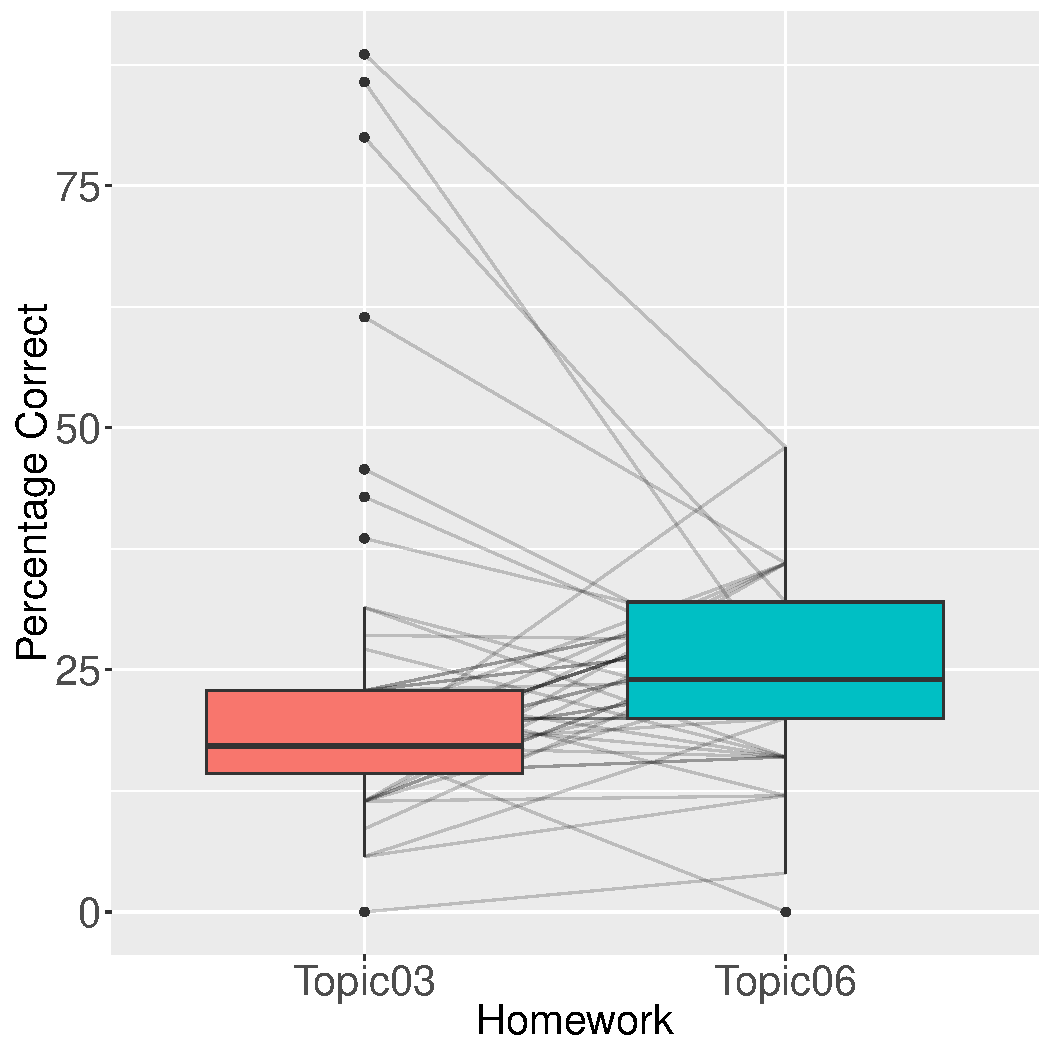
\includegraphics[width=\maxwidth]{figure/unnamed-chunk-6-1} 
\begin{marginfigure}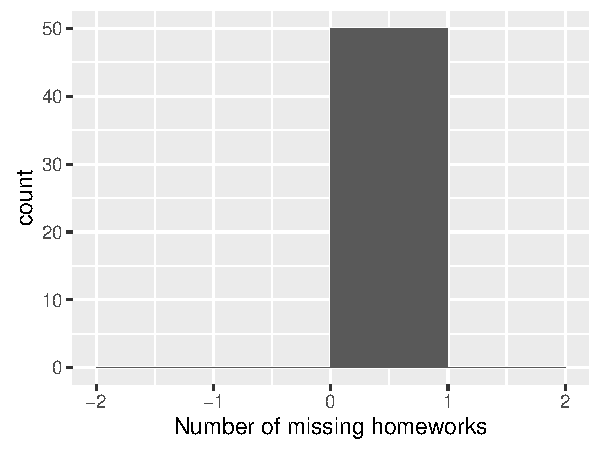
\includegraphics[width=0.95\linewidth]{Stat101_SectionAB_missinghwk}
\caption{\label{mar:missing}Histogram of the missing homeworks.}\end{marginfigure}% latex table generated in R 3.2.2 by xtable 1.8-0 package
% Sat Jan 16 13:39:58 2016
\begin{longtable}{rr}
  \hline
 & Times.Missing \\ 
  \hline
\hline
\hline
\caption{Students with missing homeworks.} 
\label{tab:missing}
\end{longtable}


\clearpage
\newpage{}
\section{Acknowledgement}
This report is generated by Xiaoyue Cheng, Dianne Cook, Lindsay Rutter, and Amy Froelich, using R-3.1.2 with package knitr, xtable and ggplot2.

\end{document}
